\documentclass[a4paper,12pt,oneside]{report}
\usepackage[utf8]{inputenc}
\usepackage[polish]{babel}
\usepackage[T1]{fontenc}
\usepackage{url}
\usepackage{graphicx}
% Dane o pracy
\author{Igor~Rzegocki}
\title{Migracja serwisu WWW z techniki PHP na Ruby~on~Rails}
\date{2008}
\pagestyle{headings}

\begin{document}
\maketitle
\tableofcontents

\chapter{Wstęp}
\label{cha:wstep}

TODO

\chapter[Technologie po stronie serwera]{Technologie serwerowe wykorzystywane w aplikacjach internetowych}
\label{cha:serwer}

Ponieważ rynek aplikacji webowych jest dzisiaj duży, wielu producentów oprogramowania chce na nim zaistnieć. Dlatego prawie każdy język proponuje rozwiązania wspomagające budowę aplikacji internetowych. Najpopularniejszymi technologiami są C\#.NET, Java, Python, Ruby oraz PHP. Oczywiście nadal można wykorzystywać Perl czy C, ale dzisiaj mało kto wybiera te języki, ze względu na istnienie lepszych rozwiązań. Jeszcze 10 lat temu dużą uwagę zwracano na wydajność. Sprzęt komputerowy był stosunkowo drogi, więc sięgano do języków niskopoziomowych, które mogły zapewnić szybkie działanie przy małym zużyciu zasobów. Jednak dzisiaj sytuacja diametralnie się zmieniła. Oczywiście wydajność jest nadal ważna, ale zmiana serwera na szybszy lub dokupienie kolejnego aby przyspieszyć działanie aplikacji nie jest już tak relatywnie drogie. Na pierwszy plan wychodzą rozwiązania, które są wygodne dla programistów i pozwalają w krótkim czasie dodać nową funkcjonalność aplikacji lub zmodyfikować istniejącą. Obecnie niewielu programistów używa tylko standardowych bibliotek do budowy aplikacji. Każdy język oferuje dodatkowe biblioteki lub całe frameworki, które ułatwiają tworzenie i rozwój aplikacji. 

Poniżej zostały scharakteryzowane wyżej wymienione języki, oraz dostępne dla nich rozwiązania.

\section{Brama CGI}
\label{sec:cgi}
Na początku wszystkie strony internetowe były statyczne. To znaczy ich autorzy tworzyli osobny plik z kodem HTML dla każdej strony. Zmiana czegokolwiek wymagała manualnej edycji kodu. Oczywiście takich stron nie można nazwać aplikacją, bardziej pasujące byłoby tu określenie publikacja.

Przełomem w tworzeniu stron i początkiem aplikacji internetowych było stworzenie w 1993 specyfikacji interfejsu CGI.

,,CGI (ang. Common Gateway Interface, ) to znormalizowany interfejs, umożliwiający komunikację pomiędzy oprogramowaniem serwera WWW a innymi programami znajdującymi się na serwerze. Zazwyczaj program serwera WWW wysyła do przeglądarki statyczne dokumenty HTML. Za pomocą programów CGI można dynamicznie (na żądanie klienta) generować dokumenty HTML uzupełniając je np. treścią pobieraną z bazy danych.''\footnote{Źródło: \url{http://pl.wikipedia.org/wiki/CGI}}

CGI jest ogniwem, które łączy serwer WWW ze skryptem CGI. Zasada działania jest bardzo prosta. Serwer WWW dostarcza dane do programu poprzez standardowe wejście, lub pod postacią zmiennych środowiskowych. Program dostarcza swój wynik na standardowe wyjście, te dane natomiast są wysyłane przez serwer do przeglądarki. 

Dzięki temu, że po drugiej stronie bramy można umieścić program twórca serwisu jest w stanie dynamicznie generować dokumenty przed wysłaniem ich do przeglądarki. Jako źródło danych  może posłużyć baza danych, następnie te dane można sformatować aby były prezentowane w sposób czytelny w oknie przeglądarki. Jako parametry program może otrzymać dane z formularza, można generować przetwarzać i zapisywać dane z ankiet i kwestionariuszy. Można dynamicznie generować obrazy takie jak wykresy czy schematy.

Co najważniejsze implementacja CGI nie jest zależna od żadnej platformy, każdy serwer WWW może zaimplementować (i przeważnie implementuje) mechanizm CGI. Programy CGI można pisać w dowolnym języku programowania, wiele języków posiada biblioteki ułatwiające obsługę interfejsu. Standard CGI\footnote{Zobacz \url{http://www.w3.org/CGI/} i \url{http://hoohoo.ncsa.uiuc.edu/cgi/}} jest dostępny za darmo i nie zmienił się od 1995 roku. 

Początkowo językami najczęściej wykorzystywanymi do współpracy z CGI były Perl oraz C. Taki wybór był w pełni uzasadniony. C był i jest bardzo popularnym językiem programowania, a jego największą zaletą jest niewątpliwie wydajność. Natomiast Perl jest językiem stworzonym do przetwarzania danych tekstowych, więc znakomicie nadaje się do generowania kodu HTML.

Mechanizm bramy CGI jest wykorzystywany do dzisiaj, jednak nie jest to najszybsza metoda komunikacji pomiędzy serwerem WWW a aplikacją obsługującą żądania HTTP. CGI zastąpiły rozszerzenia dla serwerów dedykowane dla danego języka programowania, lub nawet całe serwery dedykowane.

\section{Java}
\label{sec:java}
Java jest darmową technologią rozwijaną pod kierunkiem firmy Sun Microsystems. Kod Javy jest kompilowany do tzw. bytecode’u, który następnie jest wykonywany przez maszynę wirtualną. Jej głównymi cechami są: pełna obiektowość,  niezależność od architektury (raz stworzony bytecode może być wykonywany na wirtualnej maszynie uruchomionej na dowolnym systemie operacyjnym), sieciowość i obsługa programowania rozproszonego, niezawodność i bezpieczeństwo.

Wczesne wersje Javy były krytykowane za powolne działanie, jednak dzisiejsze wersje są o wiele szybsze i bardzo stabilne. Do budowy aplikacji webowych Sun proponuje Serwlety wykonywane po stronie serwera , a także Aplety które mogą być osadzane na stronie WWW i wykonywane przez przeglądarkę na komputerze klienta. Jedną z alternatyw jest open sourceowy framework Struts\footnote{Zobacz \url{http://struts.apache.org/}}, wspomagany przez także open sourceową bibliotekę Hibernate\footnote{Zobacz \url{http://www.hibernate.org/}} ułatwiającą obsługę bazy danych. Popularny jest także framework Spring\footnote{Zobacz \url{http://www.springframework.org/}}. Java posiada także swój serwer WWW Tomcat\footnote{Zobacz \url{http://tomcat.apache.org/}}. Budowę aplikacji ułatwiają bardzo dobre zintegrowane środowiska programistyczne (IDE) Eclipse lub NetBeans dedykowane dla tego języka.

Dużą zaletą Javy jest to, że technologia ta ma bardzo dużo zastosowań. Można w niej tworzyć takie rozwiązania, jak aplikacje okienkowe czy nawet aplikacje dedykowane dla telefonów komórkowych. Posiada bardzo rozbudowane biblioteki obsługi sieci i oprogramowania rozproszonego. Java jest językiem kompleksowym jeżeli chodzi o możliwości zastosowania. Dlatego sprawdza się wszędzie tam gdzie jeden duży system, składający się z mniejszych aplikacji i ma za zadanie pełnić wiele ról przy jednoczesnej integracji. Taki przykładem może być system ERP IFS\footnote{Zobacz \url{http://www.ifsworld.com/pl/}}, który jest w całości napisany w Javie. Zarówno cała logika biznesowa, klient okienkowy przeznaczony dla stacji roboczych, jak i część webowa w której zrealizowany jest moduł zamówień dla klientów firmy.
\begin{itemize}
\item Plusy:
  \begin{itemize}
  \item stabilność i wydajność,
  \item cena (za darmo lub open source),
  \item międzyplatformowość,
  \item mnogość możliwych rozwiązań.
  \end{itemize}
\item Minusy:
  \begin{itemize}
  \item mnogość możliwych rozwiązań,
  \item potrzeba przekompilowania kodu po każdej zmianie,
  \item rozwój aplikacji w Javie jest stosunkowo pracochłonny.
  \end{itemize}
\end{itemize}

\section{C\#.NET}
\label{sec:dotnet}
C\# jest odpowiedzią firmy Microsoft na Javę Sun'a. Podobnie jak Java jest obiektowym językiem wysokopoziomowym, kompiluje się do języka Common Intermediate Language (CIL) (podobnie jak bytecode Javy), który następnie wykonywany jest w odpowiednim środowisku uruchomieniowym. Do budowy aplikacji webowych wykorzystuje się framework .NET\footnote{Zobacz \url{http://www.microsoft.com/net/}}. Framework .NET może współpracować również z innymi językami programowania takimi jak: Visual Basic, J\#, Jscript.Net, COBOL, Fortran, Lisp, Pyton, Perl i kilka innych. .NET ma o wiele większe możliwości niż tylko aplikacje webowe. Z powodzeniem może posłużyć do budowania aplikacji okienkowych dla systemu Windows. Dedykowany serwer WWW dla aplikacji .NET to IIS\footnote{Zobacz \url{http://www.iis.net/}}, oczywiście firmy Microsoft. Firma Microsoft dostarcza także środowisko programistyczne Visual Studio.

Podobnie jak Java, framework .NET z językiem C\#  ma także szersze spektrum zastosowań. Do znanych rozwiązań należy system obsługi banku PKO~BP~S.A. czy Getin~BANK~S.A zbudowane przez krakowską firmę Vsoft\footnote{Zobacz \url{http://www.vsoft.pl/}}. Obydwa systemy obsługują większą cześć procesów w banku i posiadają także moduł banokości internetowej. Dobrym przykładem zastosowań webowych jest serwis społecznościowy MySpace\footnote{Zobacz \url{http://www.myspace.com/}}, który posiada ponad 100 milionów użytkowników na całym świecie.
\begin{itemize}
\item Plusy:
  \begin{itemize}
  \item pełne wsparcie techniczne ze strony Microsoftu,
  \item sprawdzona i stabilna technologia.
  \end{itemize}
\item Minusy:
  \begin{itemize}
  \item cena,
  \item całkowita zależność od platformy Microsoft.
  \end{itemize}
\end{itemize}

\section{PHP}
\label{sec:php}
Język PHP\footnote{Zobacz \url{http://www.php.net/}} (ang. PHP: Hypertext Preprocessor, PHP: przetwornik hipertekstu) był od początku projektowany do wykorzystania na potrzeby aplikacji webowych. Pierwotnie PHP był raczej zestawem narzędzi niż językiem, dopiero od wersji 3 można mówić o języku programowania. PHP jest językiem interpretowanym, to znaczy przy każdym uruchomieniu interpreter czyta kod źródłowy i wykonuje go. Dzięki temu każda zmiana w aplikacji ma natychmiastowe skutki. Chociaż udostępnia on możliwość programowania obiektowego, tak naprawdę jest językiem proceduralnym. Jego popularność jest bardzo duża ze względu na łatwość jego użycia. Jest całkowicie darmowy (open source), a jego interpreter jest dostępny na wiele platform. Do PHP istnieje wiele frameworków (np. Zend Framework, Zoop Framework, Symfony, Prado, CakePHP etc.), wiele bibliotek do obsługi baz danych (np. ADOdb, Propel, PEAR::DB ect.). Jednak wydaje się, że PHP nie ma przed sobą przyszłości. 
\begin{itemize}
  \item jest wiele nieścisłości w nazwach funkcji i kolejności argumentów,
  \item część standardowych bibliotek jest udostępniana proceduralnie, a część obiektowo,
  \item kompatybilność wsteczna nie pozwala na uporządkowanie języka,
  \item brak możliwości obsługi niektórych błędów powoduje zatrzymanie wykonywania aplikacji
\end{itemize}
Skrypty PHP są serwowane najczęściej za pomocą serwera Apache2.

PHP jest bardzo popularne. Nadaje się zarówno do budowy dużych aplikacji (np. \url{http://www.yahoo.com/}, \url{http://www.interia.pl/}, \url{http://facebook.com} etc.), jak i do budowy małych komponentów (np. licznik odwiedzin, księga gości etc.). Jest on bardzo często pierwszym językiem od którego programiści zaczynają przygodę z aplikacjami webowymi.
\begin{itemize}
\item Plusy:
  \begin{itemize}
  \item łatwość użycia, 
  \item popularność,
  \item dostępność,
  \item cena (open source).
  \end{itemize}
\item Minusy:
  \begin{itemize}
  \item język proceduralny,
  \item brak perspektyw rozwoju,
  \item niespójne API (ang. Application Programming Interface)
  \end{itemize}
\end{itemize}

\section{Python}
\label{sec:python}
Python\footnote{Zobacz \url{http://python.org/}} to interpretowany język programowania stworzony jako następca języka ABC\footnote{Zobacz \url{http://idhub.com/abc/}}. Jest to język zaprojektowany z myślą o jak największej produktywności oraz o prostocie i czytelności kodu. Obsługuje też typy dynamiczne oraz automatyczne zarządzanie pamięcią. Ciekawą cechą Pythona jest to, że mimo iż różne części języka są opisane i ustandaryzowane, to język sam w sobie wciąż nie ma specyfikacji. 

Python jest językiem, który wspiera różne paradygmaty programowania:
\begin{itemize}
  \item Paradygmat programowania strukturalnego
  \item Paradygmat programowania funkcjonalnego
  \item Paradygmat programowanie obiektowego
\end{itemize}

Kolejną jego cechą jest rozszerzalność. Zamiast wbudowywać wszystko w rdzeń, można łatwo dokładać napisane w C lub C++ moduły. Dzięki temu sam środek języka pozostaje mały, elastyczny i wydajny. Takie rozwiązanie wzięło się z frustracji autora językiem ABC, w którym założenia były dokładnie odwrotne \footnote{Zobacz \url{http://www.artima.com/intv/pythonP.html}}.

Python bywa często wykorzystywany w aplikacjach internetowych. Najbardziej znana to \url{http://www.youtube.com/} a z polskich \url{http://www.grono.net/}. Doczekał się również wielu frameworków -- najpopularniejsze to Django\footnote{Zobacz \url{http://www.djangoproject.com/}}, Zope\footnote{Zobacz \url{http://www.zope.org/}}, TurboGears\footnote{Zobacz \url{http://www.turbogears.org/}} i Pylons\footnote{Zobacz \url{http://www.pylonshq.com/}}.

\begin{itemize}
  \item Plusy:
  \begin{itemize}
    \item elastyczność i rozszerzalność,
    \item wydajność,
    \item wiele frameworków.
  \end{itemize}
  \item Minusy:
  \begin{itemize}
    \item duża swoboda programowania powoduje bałagan w kodzie,
    \item wymóg stosowania wcięć znacznie utrudnia stworzenie dobrego systemu szablonów.
  \end{itemize}
\end{itemize}

\section{Ruby}
\label{sec:ror}
Ruby (dosł. rubin) to interpretowany, w pełni obiektowy język programowania stworzony w 1995 roku przez Yukihiro Matsumoto. Jak twierdzi jego autor\footnote{Porównaj http://www.informit.com/articles/article.aspx?p=18225\&rl=1} Ruby został zaprojektowany dla wydajności programistów, przy zachowaniu zasady dobrego interfejsu. Ze względu na pochodzenie języka (Japonia), początkowo był on mało popularny z powodu braku angielskiej dokumentacji. Jednak dzięki Internetowi rosła jego popularność i z czasem zaczęły się pojawiać artykuły w języku angielskim a wraz z nimi społeczność skupiona wokół tego języka. Przełomem była prezentacja w 2003 roku frameworku Ruby On Rails (dosł. rubin na szynach). Rails posiadają wszystko co jest niezbędne do budowy aplikacji webowych i znakomicie nadają się do bardzo szybkiej budowy małych aplikacji a także budowania prototypów aplikacji. Interpretery Rubiego istnieją na każdą platformę. Jedyną wadą języka zdaje się być jego wydajność (podobnie jak we wczesnych wersjach Javy), którą jednak można zwiększyć wykorzystując JRuby (implementację interpretera w języku Java). Ruby posiada swoje dwa serwery WWW -- Mongrel oraz Webrick, można używać także serwera Apache za pośrednictwem CGI lub rozszerzenia mod\_ruby.

Największą aplikacja napisaną całkowicie w technologii RoR jest Basecamp\footnote{Zobacz http://www.basecamphq.com/}. Basecamp jest aplikacją wspomagającą zarządzanie projektami, która obecnie obsługuje ponad milion użytkowników. Drugą duża aplikacją jest Twitter\footnote{Zobacz http://www.twitter.com/}. Twitter jest z kolei platformą służącą do ,,mikroblogowania'' (czyli pisania wpisów nie dłuższych niż 140 znaków). Obecnie cała społeczność Ruby~on~Rails śledzi z zapartym tchem dzieje Twittera, gdyż ma on ogromne problemy wydajnościowe. Od tego jak je rozwiąże, zależy jak inwestorzy komercyjni ocenią przydatność samego frameworka.

Obecnie RoR jest wykorzystywany głównie do budowy małych aplikacji (takich jak ta prezentowana w tej pracy), oraz prototypowania aplikacji, które docelowo zostaną przepisane na bardziej wydajną platformę.
\begin{itemize}
\item Plusy:
  \begin{itemize}
  \item darmowy
  \item pełna obiektowość
  \item duże perspektywy rozwoju, 
  \item przejrzystość kodu, 
  \item bardzo prosty w nauce
  \item duża aktywna społeczność zawsze chętna do pomocy 
  \item pisanie w Rubym to naprawdę świetna zabawa
  \end{itemize}
\item Minusy:
  \begin{itemize}
  \item niska wydajność
  \item brak znanych udanych wdrożeń
  \end{itemize}
\end{itemize}

\chapter[Technologie po stronie klienta]{Technologie po stronie klienta wykorzystywane w aplikacjach internetowych}
\label{cha:klient}

\section{HTTP}
\label{sec:http}
,,HTTP (HyperText Transfer Protocol - protokół przesyłania dokumentów hypertekstowych) to protokół sieci WWW. Obecną definicję HTTP stanowi RFC~2616. Za pomocą protokołu HTTP przesyła się żądania udostępnienia dokumentów WWW, informacje o kliknięciu odnośnika oraz informacje z formularzy. Zadaniem stron WWW jest publikowanie informacji - natomiast protokół HTTP właśnie to umożliwia.''\footnote{Źródło: \url{http://pl.wikipedia.org/wiki/HTTP}}

HTTP jest to protokół zapytań i odpowiedzi pomiędzy klientem a serwerem. Jest on bardzo użyteczny, ponieważ udostępnia znormalizowany sposób komunikowania się komputerów ze sobą. Określa on formę żądań klienta dotyczących danych oraz formę odpowiedzi serwera na te żądania. Jest to protokół bezstanowy ponieważ nie zachowuje żadnych informacji o poprzednich transakcjach z klientem. Protokół definiuje osiem metod, które mogą być użyte w żądaniu HTTP:
\begin{itemize}
  \item \emph{GET} - pobranie informacji wskazanej przez URL (ang. Uniform Resource Locator, jednoznaczny wskaźnik zasobu),
  \item \emph{HEAD} - pobiera informacje o tym czy dana informacja istnieje
  \item \emph{PUT} - informacja potwierdzająca pobranie danych w postaci pliku od klienta przez serwer
  \item \emph{POST} - analogicznie jak powyżej tyle, że informacja nie musi być plikiem (np. formularze)
  \item \emph{DELETE} - żądanie usunięcia informacji -- wymagane odpowiednie uprawnienia
  \item \emph{OPTIONS} - informacje o opcjach i wymaganiach istniejących w kanale komunikacyjnym, 
  \item \emph{TRACE} - analiza i diagnostyka kanału komunikacyjnego, 
  \item \emph{CONNECT} - żądanie wykorzystywane w tunelujących serwerach proxy.
\end{itemize}

Na potrzeby przeglądania stron WWW używane są metody GET oraz POST. Natomiast cały zestaw metod protokołu daje znacznie większe możliwości i może posłużyć do kompleksowej wymiany informacji pomiędzy komputerami w sieci Internet.

\section{HTML}
\label{sec:html}
Zawartość strony internetowej jest hipertekstem, znaczy to, że użytkownik oglądając stronę internetową może podążać za hiperłączami, które przenoszą go do innych stron internetowych w ramach tego samego serwera internetowego lub innych dostępnych w ramach sieci.

,,Hipertekst to organizacja danych w postaci niezależnych leksji połączonych hiperłączami. Hipertekst cechuje nielinearność i niestrukturalność układu leksji. Oznacza to, że nie ma z góry zdefiniowanej kolejności czytania leksji, a nawigacja między nimi zależy wyłącznie od użytkownika.''\footnote{Źródło \url{http://pl.wikipedia.org/wiki/Hipertekst}}

Implementacją hipertekstu na potrzeby WWW jest język HTML 

,,HTML (HyperText Markup Language, hipertekstowy język znaczników), to język składający się ze znaczników oraz reguł ich poprawnego stosowania (gramatyki, semantyki), stosowany do pisania stron WWW. HTML jest teoretycznie aplikacją SGML, tzn. został zdefiniowany za pomocą SGML, będącego tzw. metajęzykiem (językiem służącym do definiowania innych języków).''\footnote{Źródło \url{http://pl.wikipedia.org/wiki/HTML}}

Wraz z rozwojem sieci WWW pojawiła się potrzeba rozwoju języka HTML aby posiadał on możliwość dołączania do testów danych tabelarycznych grafik czy plików multimedialnych. Kolejne wersje języka rozwijane były niezależnie przez producentów przeglądarek internetowych, co doprowadziło do częściowej  niekompatybilności wersji HTML zaimplementowanych w przeglądarkach różnych producentów. Próbą odpowiedzi na tę sytuację było stworzenie W3C\footnote{Zobacz \url{http://www.w3c.org/}} czyli World Wide Web Consortium, organizacji, która zajmuje się ustanawianiem wspólnych standardów HTML, a także innych spraw związanych z pisaniem stron WWW. Ostatnią wersją HTML jest wersja 4.01, która próbuje wydzielić zarządzanie wyglądem strony do kaskadowych arkuszy stylów (CSS). Na jakiś czas W3C zaprzestało rozwoju HTML i postanowiło dostosować język do XML (ang. eXtensible Markup Language). W wyniku powstał XHTML, dla którego istnieje tryb zgodności z HTML, który to umożliwia wyświetlenie kodu XHTML w przeglądarkach zgodnych z HTML 4.01. Zmiana ta ma zapewnić większą rozszerzalność i dostępność języka. Z tego powodu właśnie XHTML jest obecnie zalecanym standardem tworzenia stron WWW. Obecną najnowszą wersją hipertekstu na potrzeby stron WWW jest XHTML 1.1\footnote{Zobacz \url{http://www.w3.org/TR/xhtml11/}}, a dla niego arkusze styli CSS 2.1\footnote{Zobacz \url{http://www.w3.org/TR/REC-CSS2/}}. Kolejną wersją języka (X)HTML miał być XHTML 2.0, jednak ta droga rozwoju została ostatecznie uznana za nietrafioną i rozwój XHTML 2.0 został zarzucony na rzecz HTML 5\footnote{Zobacz \url{http://www.w3.org/html/wg/html5/}}, nad rozwojem którego trwają obecnie intensywne prace.

\section{CSS}
\label{sec:css}
,,Kaskadowe arkusze stylów (ang. Cascading Style Sheets, CSS) to język służący do opisu formy prezentacji (wyświetlania) stron WWW. CSS został opracowany przez organizację W3C w 1996 r. jako potomek języka DSSSL przeznaczony do używania w połączeniu z SGML-em. Pierwszy szkic CSS zaproponował w 1994 r. Håkon Wium Lie.\footnote{Zobacz http://www.w3.org/People/howcome/p/cascade.html}''

CSS jest wykorzystywany aby wspomóc czytniki stron WWW w definiowaniu kolorów, czcionek, układów i innych aspektów prezentacji dokumentu. Głównym założeniem projektowym była separacja warstwy treści (zapisanej w HTML albo w podobnym języku znaczników) od warstwy prezentacji (zapisanej w CSS). Taka separacja znacznie podnosi dostępność treści, zapewnia dużo większą elastyczność i kontrolę nad aspektami prezentacyjnymi dokumentu. Dodatkowo redukuje powtarzalność w warstwie dokumentu (jeżeli chcemy np. aby wszystkie nagłówki były koloru zielonego, nie musimy go nadawać każdemu z nich z osobna). CSS pozwala również na to, aby ta sama treść była wyświetlana w różny sposób na różnych urządzeniach (np. inaczej będziemy wyświetlać stronę na ekranie komputera, inaczej na telefonie komórkowym a jeszcze inaczej w wersji do druki). CSS określa też priorytety z jakimi należy nakładać kolejne właściwości. Najnowszą wersją CSS jest obecnia wersja 2.1 -- trwają jednak prace, nad wersją trzecią\footnote{Zobacz \url{http://www.w3.org/Style/CSS/current-work}}.

\section{JavaScript}
\label{sec:javascript}
JavaScript jest skryptowym językiem programowania, który został opracowany przez firmę Netscape na potrzeby stron internetowych. JavaScript jest wersją standaryzowanego języka ECMAScript\footnote{Pełny standard \url{http://www.ecma-international.org/publications/files/ECMA-ST/Ecma-262.pdf}}.

Nazwa nasuwa skojarzenie z językiem Java, jednak oba języki nie mają ze sobą wiele wspólnego, oprócz tego że ich składnia jest zaczerpnięta z języka C. W połączeniu z Document Object Model\footnote{Zobacz \url{http://www.w3.org/DOM/}} JavaScript stał się o wiele bardziej potężną technologią niż przewidywali jej twórcy. Po załadowaniu strony programista ma możliwość manipulacji strukturą dokumentu (załadowanej do przeglądarki strony), może także tworzyć funkcje, które reagują na zdarzenia występujące w oknie przeglądarki (ruchy, klikniecie myszką, naciśnięcie klawisza na klawiaturze etc.). Połączenie HTML ze skryptami języka JavaScript nazywane jest Dynamic HTML (DHTML), czyli dynamiczny HTML, aby uwydatnić różnicę ze statycznymi stronami HTML. 
Przełomem w DHTML było udostępnienie obiektu XMLHttpRequest (XHR). XHR umożliwia wysyłanie żądań HTTP z poziomu języka JavaScript już po załadowaniu się strony internetowej w trakcie interakcji z użytkownikiem. Otrzymane odpowiedzi serwera są wówczas wykorzystywane do modyfikacji załadowanego dokumentu. Możliwość asynchronicznego wykonywania żądań sprawia, że są one wykonywane w tle i nie przerywają interakcji użytkownika ze stroną, dynamicznie ją zmieniając. Technika wykorzystania obiektu XHR została nazwana AJAX (ang. Asynchronous JavaScript and XML, asynchroniczny JavaScript i XML) . Dzisiaj każda przeglądarka udostępnia XHR. AJAX sprawdza się tam gdzie nie ma potrzeby przeładowywania całej strony, a tylko jej części lub gdzie w ogóle nie trzeba dokonywać przeładowania a jedynie wysłać informację do serwera WWW. AJAX oszczędza czas użytkownika (w trakcie doładowywania informacji może on przeglądać stronę, która dalej jest dla niego dostępna) oraz zmniejsza obciążenie serwera (doładowywanie tylko części informacji zamiast całej strony ogranicza ilość danych wysyłanych do przeglądarki). 

\section{Przeglądarki Internetowe}
\label{sec:przegladarki}

,,Przeglądarka internetowa – program komputerowy, który służy do pobierania i wyświetlania dokumentów HTML/XHTML/XML z serwerów internetowych, a także plików multimedialnych''\footnote{Źródło \url{http://pl.wikipedia.org/wiki/Przeglądarka\_internetowa}}.

Na rynku istnieje wiele przeglądarek, jednak tak naprawdę nie jest istotna ich nazwa a silnik jaki wykorzystują do wyświetlania stron. Cztery najważniejsze silniki to: Trident (Internet Explorer), Gecko (np. Firefox, Netscape, Flock, SeaMonkey, Camino etc.), KHTML/WebKit (np. Konqueror, Safari), oraz Presto (Opera). Jeżeli chodzi o udział przeglądarek w rynku przedstawia się jak na rysunku \ref{fig:przegladarki}
\begin{figure}
\begin{center}
  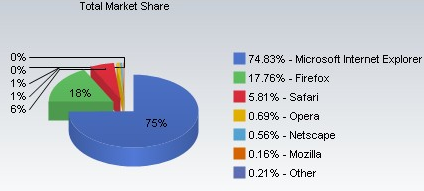
\includegraphics{browsers.png}
  \caption{
  Wykres 1. Udział procentowy w rynku przeglądarek internetowych.\newline
  \emph{Źródło: http://marketshare.hitslink.com/report.aspx?qprid=0}
  \label{fig:przegladarki}
  }
  \end{center}
\end{figure}

Niestety silniki nie są ze sobą ze sobą kompatybilne, każdy trochę inaczej interpretuje HTML, CSS, JavaScript, nie wszystkie mają wbudowane najnowsze technologie w tym samym stopniu. Największe trudności sprawia programistom przeglądarka Internet Explorer w wersji 6, która zajmuje największą część rynku i zarazem jest najbardziej przestarzałą (2001 r.).  Ta wersja jest niezgodna ze standardami zatwierdzonymi przez W3C i posiada wiele błędów. Niestety przeglądarka IE 6 wygrała pierwszą ,,wojnę przeglądarek''\footnote{Zobacz \url{http://en.wikipedia.org/wiki/Browser\_wars}} i niemalże zmonopolizowała rynek. Następna wersja Internet Explorera (wersja 7) pojawiła się dopiero pod koniec 2006 roku. Zanim wersja 6 zniknie z rynku minie jeszcze kilka lat, w czasie których rozwój aplikacji po stronie klienta będzie ograniczony możliwościami tej przeglądarki.

\chapter[Rozwiązania koncepcyjne]{Koncepcje spotykane w aplikacjach internetowych}
\label{cha:koncepcje}

\section{Model-view-controller}
\label{sec:mvc}
MVC (ang. Model-view-controller, model-widok-kontroler) to wzorzec projektowy stosowany szeroko w informatyce, niemniej największą popularność zyskał w Internecie. Odpowiednie użycie wzorca oddziela logikę biznesową od warstwy prezentacji, co w efekcie przekłada się na możliwość zmiany wyglądu aplikacji bez wpływu na logikę biznesową i odwrotnie. W MVC Model reprezentuje informacje o aplikacji i założeniach biznesowych użytych w celu obróbki danych. Widok, odpowiada za elementy UI (ang. User Interface, interfejs użytkownika) takie jak tekst, listy, pola wyboru etc. Kontroler spaja wszystko w całość pośrednicząc między Modelem a Widokiem i zajmując się sterowaniem.

\subsection{Krótka Historia}
\label{subsec:mvc-historia}
Wzorzec został po raz pierwszy opisany w 1979~r.\footnote{Zobacz \url{http://heim.ifi.uio.no/~trygver/themes/mvc/mvc-index.html}} przez Trygve Reenskaug wtedy pracującegp w XEROX~PARC nad językiem Smalltalk\footnote{Zobacz \url{http://www.smalltalk.org/}} Oryginalna implementacja została dokładnie opisana w dokumencie \emph{Applications Programming in Smalltalk-80: How to use Model-View-Controller.}\footnote{Zobacz \url{http://st-www.cs.uiuc.edu/users/smarch/st-docs/mvc.html}}.

Po pewnym czasie, powstało wiele wariacji na temat koncepcji, dość wspomnieć o wzorcu Model-view-presenter, który powstał początkiem lat 90 i został zaprojektowany jako następca MVC. Nie zmienia to faktu, że MVC trzyma się mocno i wciąż znajduje szerokie zastosowanie.

\subsection{Opis wzorca}
\label{subsec:mvc-opis}
Dość powszechnie stosowaniem rozwiązaniem jest dzielenie aplikacji na warstwę prezentacji i warstwę logiczną. MVC idzie o krok dalej, dzieląc warstwę prezentacji na Widok i Kontroler. Kładzie on też większy nacisk na architekturę aplikacji niż typowy wzorzec projektowy. Trzy jego główne elementy to:
\begin{itemize}
  \item \emph{Model} - Specyficzna dla każdego projektu reprezentacja informacji, na których działa aplikacja. Jest to DSL (ang. Domain Specific Language, zob.~r.~\ref{sec:dsl} str.~\pageref{sec:dsl}), który opisuje i operuje na surowych danych (np. obliczenie czy dzisiaj użytkownik obchodzi urodziny, kosztu wszystkich towarów w koszyku etc.). Wiele aplikacji wykorzystuje ściśle określony mechanizm przechowywania danych (w przypadku aplikacji internetowych, prawie zawsze jest to baza danych). MVC sam w sobie, nie określa metody przechowywania danych, ponieważ założenie jest takie, że danymi zajmuje się model.
  \item \emph{Widok} - Przedstawia dane z modelu w postaci czytelnej dla użytkownika. MVC nie definiuje ścisłej relacji ilościowej pomiędzy Modelami a Widokami, co oznacza, że jeden Model może obsługiwać wiele widoków jak i jeden Widok może otrzymywać dane od wielu Modeli.
  \item \emph{Kontroler} - Odpowiada za proces interakcji między aplikacją użytkownikiem. Pobiera ,,zapytania'' od użytkownika i przekazuje je Modelowi. Następnie zwraca użytkownikowi nowy widok z nowymi informacjami. Może również dokonywać zmian w samym Modelu.
\end{itemize}

\subsection{Zastosowanie w aplikacjach internetowych}
\label{subsec:mvc-web}
MVC często znajduje zastosowanie w aplikacjach internetowych, gdzie widokiem jest aktualnie wyświetlana strona WWW, a kontroler to kod, który pobiera dane dynamiczne i wypełnia nimi HTML. Model z kolei reprezentuje dane (zazwyczaj przechowywane w bazie danych lub plikach XML) oraz reguły biznesowe, które zamieniają te dane na informację przedstawianą potem użytkownikowi.

Mimo, że MVC jest dostarczany w wielu frameworkach, z których każdy ma odmienny pomysł na jego implementację, generalna zasada jest taka sama:
\begin{enumerate}
  \item Użytkownik wykonuje jakąś akcję w UI (np. wciska guzik).
  \item Kontroler obsługuje nadchodzące wywołanie, często wykorzystując jakąs metodę lub odwołanie.
  \item Kontroler informuje model o akcji użytkownika, czasami również modyfikuje jego stan (np. Kontroler uaktualnia zawartość koszyka).
  \item Widok wykorzystuje model (pośrednio) do wygenerowania odpowiedniego interfejsu użytkownika (np. wyświetla tabelkę z zakupami). Widok pobiera dane z modelu, ale sam model nic nie wie o Widoku.
  \item UI oczekuje na kolejną akcję, co rozpoczyna cały cykl od początku.
\end{enumerate}

Rozdzielając Modele od Widoków, MVC znacznie zmniejsza skomplikowanie architektury programu i zwiększa przejrzystość i elastyczność.

\section{Object-relational mapping}
\label{sec:orm}
Mapowanie obiektowo-relacyjne (z ang. Object-relational mapping) jest techniką programistyczną stosowaną do konwersji danych przy niekompatybilnych ze sobą relacyjnych baz danych i obiektowo zorientowanych językach programowania. W efekcie otrzymywany jest ,,wirtualny obiekt bazy danych'', który może być następnie użyty na poziomie kodu zadanego języka programowania. Istnieją zarówno darmowe jak i komercyjne rozwiązanie ORM, niemniej sporo programistów wciąż tworzy swoje rozwiązania.

\subsection{Opis problemu}
\label{subsec:orm-problem}
Zarządzanie danymi w programowaniu obiektowym zazwyczaj jest rozwiązane jako manipulowanie różnego rodzaju obiektami, które prawie nigdy nie są wielkościami skalarnymi. Dla przykładu, dany jest obiekt reprezentujący osobę w książce teleadresowej. Osoba taka, może mieć kilka telefonów i kilka adresów (zameldowania, zamieszkania etc.). Obiekt reprezentujący taką osobę miałby kilka ,,slotów'', które zawierałyby kolejno, dane osobowe, listę telefonów i listę adresów. Oczywiście, lista telefonów może z kolei zawierać obiekty numerów telefonów (z osobnym slotem, na operatora, numer kierunkowy etc.), lista adresów obiekt adresu itd. Dodatkowo, wszystkie te obiekty miałyby swoje własne metody, np. do zwracania telefonu domowego, preferowanego adresu itd.

Z drugiej strony, bazy danych mogą przechowywać tylko dane skalarne zorganizowane w tabelach.

Programista musi więc albo zorganizować podobne wartości obiektów jako dane dla tabeli, albo całkowicie uprościć strukturę kodu, do poziomu wartości skalarnych aby potem bezproblemowo umieszczać je w bazie. Podejście ORM wykorzystuje pierwsze rozwiązanie.

Cały problem polega na takiej organizacji tych obiektów, aby potem dało się je łatwo zapisać do bazy, jednocześnie nie tracąc samej struktury obiektu (w celu późniejszego odczytu). Obiekty takie muszą być więc przenaszalne między kodem a bazą danych.

\subsection{Implementacje}
\label{subsec:orm-implementacje}
Najpowszechniej stosowanym rozwiązaniem jest relacyjna baza danych, która poprzedziła narodziny ORM w 1990 r. Relacyjne bazy danych, wykorzystują serie tabel do organizacji danych. Dane w różnych tabelach są ze sobą powiązane przy pomocy kluczy założonych na całe kolumny, a nie na poszczególne wartości. Może się okazać, że dane przechowywane w jednym obiekcie muszą być rozłożone na kilka tabel.

ORM powinien systemacznie przewidywać jakie tabele będą potrzebne do zapisania określonych obiektów i generować odpowiednie zapytania SQL. Różnice między sposobem prezentacji danych w modelu obiektowo zorientowanym (w takich językach jak Java, C\# czy Ruby) a sposobem ich przechowywania w relacyjnej bazie danych (takiej jak Oracle czy PostgreSQL), pociągają za sobą następujące problemy:
\begin{itemize}
  \item Wydajność,
  \item Skalowalność,
  \item Zarządzanie operacjami typu CRUD (patrz rozdz.~\ref{sec:crud}, str.~\pageref{sec:crud}) dla bardziej skomplikowanych relacji,
  \item Uproszczenie i spójność kodu konieczna przy szybkim tworzeniu aplikacji,
  \item Zarządzanie i elastyczność kodu.
\end{itemize}

Prawdziwą wartością ORM jest przedewszystkim oszczędność czasu i uproszczenie kodu (wszystkie skomplikowane operacje bazodanowe ORM załatwia za programistę). Dodatkowo ORM zwiększa wydajność i skalowalność oraz minimalizuje problemy niekompatybilności architektur (dobry ORM obsługuje większość obecnie stosowanych systemów baz danych).

Powstało sporo aplikacji ORM, które dostarczając zestaw klas i bibliotek autmatyzują proces mapowania i odciążają programistę. Po podaniu im listy tabel w bazie, same wygenerują odpowiednie obiekty i relacje między nimi. Wracając do poprzedniego przykładu -- pytając taki obiekt o numer telefonu, w tle nastąpi utworzenie zapytania SQL, wysłanie go do bazy, przetworzenie wyniku a następnie konwersja do postaci zgodnej z obiektem.

Z punktu widzenia programisty, nie powinno go zajmować jak to wszystko się odbywa -- powinien tylko wiedzieć, że zapisanie danej do obiektu, skutkuje zapisaniem jej w bazie.

W praktyce nie jest to takie proste. Nie jest możliwe stuprocentowe zmapowanie wszystkich możliwych kombinacji zapytań. Wszystkie ORM mają margines błędu, który użytkownik może zniwelować tylko poprzez bezpośrednie wysłanie zapytania SQL do bazy. Dodatkowo, cały proces mapowania i unifikacji zapytań pociąga za sobą spadek wydajności (zapytania SQL z poziomu ORM są tworzone z myślą o jak największej elastyczności i uniwersalności, więc niekoniecznie muszą być najszybsze dla konkretnego przypadku).

\subsection{Zastosowanie w aplikacjach internetowych}
\label{subsec:orm-web}
Koncepcja ORM jest wykorzystywana we wszystkich nowoczesnych frameworkach webowych, ponieważ ściąga z programisty konieczność dbania o spójność danych w bazie, utrzymywania i rozłączania połączeń etc. Nie bez znaczenia jest też wsparcie dla różnych architektur bazodanowych. Często dzieje się tak, że po przeniesieniu aplikacji na nowy serwer okazuje się, że baza danych zmieniła się. Wtedy wystarczy tylko jedna zmiana w pliku konfiguracyjnym, a całość powinna zadziałać automatycznie.

Drugą, znaczącą zaletą jest to, że ORM wymusza spójność kodu (przynajmniej w kwestii obsługi bazy danych) -- oznacza to, że przy projektach pisanych przez wielu programistów, jest znacznie mniej niespójności i nieścisłości -- wszyscy trzymają się jednej konwencji.

\section{Representational State Transfer}
\label{sec:rest}
REST (ang. REpresentional State Transfer, reprezentacja stanu transferu) jest to styl w architekturze programowania przeznaczony dla multimedialnych systemów rozproszonych takich jak World Wide Web. Określenia ,,Representional state transfer'' i ,,REST'' zostały pierwszy raz zaprezentowane w 2000 roku na rozprawie doktorskiej, którą przeprowadzał Roy Fielding\footnote{Zobacz http://www.ics.uci.edu/~fielding/pubs/dissertation/rest\_arch\_style.htm} -- jeden z głównych autorów specyfikacji protokołu HTTP. Zwroty te, szybko rozpowszechniły się wśród sieciowej społeczności.

REST ściśle odnosi się do założeń sieciowych, które określają jak zasoby są definiowane i adresowane. Określenie to, jest też często używane w luźnym sensie, do opisania jakiegokolwiek prostego interfejsu, który przesyła informacje określone w danej domenie (patrz rozdz.~\ref{sec:dsl}, str.~\pageref{sec:dsl}) poprzez protokół HTTP wraz z dodatkową warstwą wiadomości, taką jak SOAP czy też kontrolą sesji wykorzystującą ,,ciasteczka''. Oba te określenia mogą budzić konflikt, jak i się uzupełniać. Jest możliwe zaprojektowanie dużej, skomplikowanej aplikacji w metodologii REST, jednocześnie nie używając HTTP i nie łączac jej z WWW. Jednakże, jest także możliwe zbudowanie prostej aplikacji XML+HTTP, która zupełnie nie spełnia założeń REST. Te różnice w używaniu terminu ,,REST'', często prowadzą do pewnego zakłopotania w technicznych dyskusjach.

Systemy, które spełniają założenia REST, często bywają określane jako ,,RESTful''.

\subsection{Założenia}
\label{sub:rest-zalozenia}
Najważniejszym założeniem w REST jest istnienie zasobów (źródeł określonej informacji), z których każdy może być zaadresowany używając globalnego odnośnika URI (ang. Uniform Resource Identifier, jednoznaczny identyfikator zasobu). Aby modyfikować te zasoby, komponenty sieci (klienci i serwery) komunikują się między sobą przez zestandarazywany interfejs (np. HTTP) i wymieniają między sobą reprezentacje tych zasobów (dokumenty zawierające określone informacje). Dla przykładu zasób ,,okrąg'' może przyjmować i zwracać reprezentację w postaci współrzędnych środka i promienia, skonwertowaną do formatu SVG, ale może też to być plik tekstowy zawierający trzy współrzędne po średniku, które lężąc na tym okręgu definiują go jednoznacznie.

Orędownicy REST utrzymują, że skalowalność i rozwój sieci są bezpośrednią przyczyną kilku kluczowych założeń:
\begin{itemize}
  \item Stany i funkcjonalności aplikacji są podzielone między zasoby,
  \item Każdy zasób jest unikalnie adresowalny używając uniwersalnej składni wykorzystywanej do tworzenia odnośników,
  \item Wszystkie zasoby dzielą jednolity interfejs do transportu stanów pomiędzy klientem a zasobem, zawierający:
  \begin{itemize}
    \item Ograniczony zestaw dobrze opisanych rozkazów,
    \item Ograniczony zestaw typów danych, może jednak być wysłany w ramach ,,kodu na żądanie''.
  \end{itemize}
  \item Protokół, którego cechami są:
  \begin{itemize}
    \item Klient-serwer,
    \item Bezstanowość,
    \item Cacheowalność,
    \item Warstwowość.
  \end{itemize}
\end{itemize}

\subsection{Zastosowanie w aplikacjach internetowych}
\label{rest:web}

World Wide Web jest kluczowym przykładem projektu typu ,,RESTful''. Większość założeń WWW, pokrywa się z założeniami REST. Sieć opiera się na protokole HTTP, prezentacji treści w postaci dokumentów HTML oraz różnych innych technologii internetowych, jak np. DNS (Domain Name System, system nazw domenowych).

HTML może zawierać JavaScript i applety aby wspierać kod na żądanie, oraz posiada wbudowaną obsługę hyperlinków.

HTTP jest jednolitym interfejsem dostępu do zasobów, który zawiera URI, metody, kody stanu, nagłówki i zawartość opisaną MIME type (ang. Multipurpose Internet Mail Extensions, rozszerzenia poczty internetowej stosowane do różnych celów).

Najważniejszymi metodami HTTP są POST, GET, PUT i DELETE (patrz rozdz.~\ref{sec:http}, str.~\pageref{sec:http}). Są one często porównywane do CREATE, READ, UPDATE i DELETE (CRUD, patrz rozdz.~\ref{sec:crud}, str.~\pageref{sec:crud}), które to pojęcia mają zastosowanie w bazach danych.

\begin{table}[h]
  \begin{center}
    \begin{tabular}{|l|l|}\hline
    HTTP   & CRUD \\\hline
    POST   & Create, Update, Delete \\
    GET    & Read \\
    PUT    & Create, Update \\
    DELETE & Delete \\\hline
    \end{tabular}
  \caption{Porównanie zapytań HTTP z koncepcją CRUD\label{rest:crud}}
  \end{center}
\end{table}

HTTP spełnia jedno z założen REST -- jest bezstanowy. Każda wiadomość zawiera wszystkie informacje niezbędne do identyfikacji zapytania. W efekcie czego, ani klient ani serwer nie muszą pamiętać żadnych stanów informacyjnych pomiędzy wiadomościami. Każdy stan w którym jest serwer, może być zamodelowany jako zasób.

Ta bezstanowość może być naruszona w HTTP, kiedy używamy ciasteczek do podtrzymywania sesji. Używanie ciasteczek często wiąże się z naruszeniami polityki prywatności i problemami bezpieczeństwa. Dodatkowo, pojawia się wiele nieścisłości i błędów jeśli do problemów z ciasteczkami dołożymy jeszcze obecność przycisku ,,wstecz'' w przeglądarce.

Nie bez znaczenia jest też fakt, że hipertekst HTML tak naprawdę pozwala tylko na użycie zapytań typu ,,GET''. Dodatkowo jest jeszcze dostępny ,,POST'' dzięki formularzom. Pozostałe metody HTTP nie są wspierane ani przez HTML~4.01 ani XHTML~1.0.\footnote{Więcej informacji na http://www.w3.org/TR/2007/REC-wsdl20-adjuncts-20070626/\#\_http\_binding\_default\_rule\_method}

\section{Domain Specific Language}
\label{sec:dsl}
DSL (z ang. Domain Specific Language, język określonego przeznaczenia) to język zaprojektowany w ściśle określonym celu. W przeciwieństwie do języków ogólnego przeznaczenia takich jak Java czy C, których zadaniem jest uniwersalność i możliwość zastosowania w jak największej liczbie przypadków, DSLe są projektowane tylko w jednym, ściśle określonym celu. Przykładem DSLa jest np. język SQL - zaprojektowany tylko i wyłącznie do obsługi baz danych. Termin DSL nie jest terminem nowym, jednak dopiero ostatnio zyskał sobie sporą popularność. Powodem tego jest znaczny wzrost mocy obliczeniowej komputerów oraz elastyczność nowych języków generalnego przeznaczenia, która umożliwia pisanie własnych DSL.

\subsection{Przykłady zastosowań}
\label{sub:zastosowania}

Można wykazać conajmniej kilka przykładów zastosowań dla DSL:
\begin{enumerate}
  \item wykorzystywanie samodzielnych aplikacji wywoływanych przez bezpośrednią akcję użytkownika (najczęściej z poziomu linii poleceń lub pliku Makefile), np. zestaw narzędzi GraphViz
  \item DSL, które są zaimplementowane przy użyciu systemów makr, a następnie są konwertowane lub rozszerzane do trybu zgodności z nadrzędnym językiem programowania ogólnego przeznacznia, podczas fazy kompilacji lub interpretowania
  \item DSL w całości napisane w języku programowania ogólnego przeznaczenia (takim jak C lub Perl), mające na celu wykonywanie określonych operacji i zwracanie danych, które język nadrzędny jest w stanie zrozumieć i przetworzyć. Generalnie, taki DSL można rozumieć jako język programowania szczególnego przeznaczenia napisany w języku programowania ogólnego przeznaczenia.
  \item DSL, które są częścią aplikacji w której pracują -- dobrym przykładem są tu różnego rodzaju systemy makr w arkuszach kalkulacyjnych, wykorzystywane do uruchamiania specyficznych funkcji napisanych przez użytkownika, lub tworzone dynamicznie przez samą aplikację.
\end{enumerate}

Wiele DSL może być używane w kilku powyższych przypadkach naraz.

\subsection{Zastosowanie w aplikacjach internetowych}
\label{dsl:web}
W aplikacjach internetowych DSL znalazły szerokie zastosowanie przy zadaniach często powtarzających się, takich jak na przykład tworzenie modeli, testy czy obsługa baz danych. Nie można również zapomnieć o najważniejszym z DSL z punktu widzenia WWW -- o SQL. Bez niego istnienie większości serwisów internetowych byłoby praktycznie niemożliwe. DSL świetnie też się sprawdzają w całej otoczce okołoaplikacyjnej. Używając ich, można zautomatyzować procesy takie jak:
\begin{itemize}
  \item Wysyłanie aplikacji na serwer
  \item Synchronizacja z systemem kontroli wersji np. SVN (z ang. SubVersioN)
  \item Testowanie aplikacji oraz jej poszczególnych komponentów
  \item Wiele różnych akcji związanych z przejściem z trybu developerskiego na produkcyjny, jak np.:
  \begin{itemize}
    \item Kompresja i obfuskacja (zaciemnienie) plików JavaScript
    \item Kompresja CSS
    \item Usuwanie informacji o gammie z plików PNG (ang. Portable Network Graphics, przenośna grafika sieciowa)
    \item Zmiany nazw plików aby zostały ponownie pobrane (dotyczy to w szczególności serwisów, gdzie wymuszany jest nieskończony czas cacheowania plików przez przeglądarkę)
    \item Czyszczenie różnych pozostałości developerskich (stare, skompilowane pliki szablonów, logi, etc.)
  \end{itemize}
\end{itemize}

\section{Create, Read, Update and Delete}
\label{sec:crud}
CRUD (Create, read, update and delete -- utwórz, odczytaj, popraw i skasuj) są to cztery podstawowe funkcje dotyczące operacji na danych, najważniejszej czynności w całej informatyce. Czasami w skrócie tym, zamiast ,,read'' używa się ,,restore'' a zamiast ,,delete'' -- ,,destroy''. Często jest stosowany przy opisywaniu operacji na bazach danych lub przy opisie interfejsów.

\subsection{CRUD w relacyjnych bazach danych}
\label{sub:crud-db}
Akronim CRUD jest często odnoszony do relacyjnych baz danych, ponieważ te cztery operacje determinują zupełność takiej bazy danych. Każda litera akronimu, może zostać przedstawiona jako odpowiednia funkcja SQL:
\begin{table}[h]
  \begin{center}
    \begin{tabular}{|l|l|} \hline
    Operacja         & SQL \\\hline
    Create           & INSERT \\
    Read (Retrieve)  & SELECT \\
    Update           & UPDATE \\
    Delete (Destroy) & DELETE \\\hline
    \end{tabular}
    \caption{Mapa akronimu CRUD na zapytania SQL\label{crud:sql}}
  \end{center}
\end{table}
Pomimo iż CRUD głównie odnosi się do relacyjnych baz danych, często jest też stosowany w odniesieniu do obiektorych baz danych, XMLowych baz danych, plików tekstowych, nośników informacji etc.

\subsection{Zastosowanie w aplikacjach internetowych}
\label{crud:web}
W aplikacjach internetowych, CRUD odnosi się do samego interfejsu. Dla przykładu, jeśli tworzona jest książka teleadresowa, podstawową jednostką danych jest informacja o kontakcie. Jako niezbędne minimum, aplikacja musi:

\begin{itemize}
  \item Utworzyć lub dodać nowy kontakt (Create)
  \item Wyświetlić istniejące wpisy (Read)
  \item Zmieniać niektóre informacje (Update)
  \item Usuwać niepotrzebne kontakty (Delete)
\end{itemize}

Bez którejkolwiek z powyższych operacji, aplikacja nie może być uznana za kompletną. Zasada ta, też jest podwaliną każdego dobrego frameworka, gdyż zautomatyzowanie jej, znacznie skraca czas tworzenia programu.

\section{Don't Repeat Yourself}
\label{sec:dry}
DRY (z ang. Don't Repeat Yourself, nie powtarzaj się) jest filozofią, której celem nadrzędnym jest zredukowanie duplikatów. Występuje głównie w informatyce. DRY zakłada, że ta sama informacja nie powinna być powielana w ramach jednego projektu, gdyż taka duplikacja znacznie utrodnia zmiany, zmniejsza czytelność i prowadzi do niespójności. Don't Repeat Yourself jest głównym przykazaniem książki \emph{The Pragmatic Programmer}\footnote{TODO: BIBLIOGRAFIA}, której autorami są Andy Hunt i Dave Thomas. W publikacji tej, zalecają, aby używać jej w jak najszerszym zakresie, włączając ,,schematy baz danych, plany testów, budowany system a nawet dokumentacje''\footnote{Wywiad Billa Vennersa z Dave Thomasem \emph{Orthogonality and the DRY Principle}, zob.~\url{http://www.artima.com/intv/dry.html}}. Kiedy reguła DRY zostanie pomyślnie wdrożona w system, jakakolwiek zmiana jakiegoś elementu w kodzie, nie wpłynie w żaden sposób na elementy nie będące z nim logicznie połączone. Dodatkowo, wszystkie elementy logicznie połączone ze zmienionym, zmienią się w sposób przewidywalny i wciąż będą ze sobą zsynchronizowane.

\subsection{Kiedy DRY może się nie sprawdzić}
\label{sub:dry-not}
Reguła DRY nie zawsze się sprawdza i w niektórych przypadkach, lepiej z niej zrezygnować:
\begin{itemize}
  \item W małych projektach, albo prostych skryptach, wysiłek jaki trzebaby było włożyć aby trzymać się reguły DRY, byłby znacznie większy niż proste napisanie dwóch kopii tej samej danej w różnych miejscach,
  \item Wymuszanie DRY w projektach, w których najważniejszą rolę w tworzeniu treści pełni społeczność (np. wikipedia), mogłoby znacznie ostudzić zapał ludzi do tworzenia nowych wpisów,
  \item Zarządzanie projektami i kontrolą wersji pozwala (a nawet) zaleca tworzenie kilku kopii, bez wykorzystywania DRY. Dla przykładu, bardzo dobrym nawykiem jest tworzenie trzech środowisk dla jednej aplikacji -- produkcyjnego, testowego i deweloperskiego. Dzięki temu mamy pewność, że rozwojowy albo testowy kod, nie będzie miał wpływu na stabilne wersje produkcyjne,
  \item Dokumentacja dla użytkowników końcowych (od komentarzy w kodzie, do drukowanych instrukcji) zawiera typowe informacje opisujące pewnie funkcjonalności kodu, przeznaczone dla ludzi, którzy nie potrzebują lub nie mają czasu analizować całego listingu programu. Niestety DRY zakłada, że jeśli taka dokumentacja nie stanowi jakiejś wartości dla samego kodu (a nie dla użytkowników), to powinna być generowana a nie pisana,
  \item Generatory kodu źródłowego - niepowtarzalność będzie skuteczna dla generatora samego w sobie, ale nie musi już być konieczna dla samego wygenerowanego źródła, które jest używane automatycznie i nikt nie będzie do niego zaglądał ani go zmieniał.
\end{itemize}

\subsection{Zastosowanie w aplikacjach internetowych}
\label{dry:web}
Reguła DRY świetnie sprawdza się we wszystkich projektach programistycznych, ale największe uznanie znalazła właśnie wśród programistów aplikacji internetowych. Specyfika internetu jest inna niż desktopu -- wszystkie zmiany zachodzą dużo szybciej. Czas życia przeciętnego projektu internetowego to kilka lat i w tym czasie musi on podlegać ciągłemu rozwojowi i przemianom. Gdyby nie DRY, zmiany zachodziły by dużo wolniej, byłyby dużo trudniejsze do przeprowadzenia i pochłaniałyby więcej środków. Filozofia DRY (oczywiście w pełni respektowana) wymusza na programistach WWW porządek w kodzie dzięki czemu taka aplikacja jest w stanie szybko przystosować się do zmiennych warunków rynkowych.

\section{Convention over Configuration}
\label{sec:coc}
Convention over Configuration (konwencje ponad konfiguracje) jest jedną metodologii projektowania oprogramowania, która dąży do osiągnięcia minimalizacji ilości decyzji jakie muszą podjąć deweloperzy, zyskując dzięki temu prostotę bez utraty elastyczności.

Sformułowanie samo w sobie oznacza, ze programista musi rozpatrywać tylko niekonwencjonalne aspekty aplikacji. Dla przykładu, jeśli dana jest klasa \emph{Sprzedaż} obsługująca model, to przypisana jej tabela jest domyślnie również nazwana ,,sprzedaż''. Jeżeli teraz nie zostanie naruszona konwencja (czyli np. tabela nie zostanie nazwana ,,sprzedaż\_produktów''), to programista nie musi nigdzie określać nazwy tabeli i potem odwoływać się do niej w innych miejscach.

Im więcej dobrych konwencji w kodzie, tym na wyższym poziomie abstrakcji może się skupić programista, co oznacza, że mocniej zajmuje się aspektami logicznymi zagadnienia, a nie technicznymi.

\subsection{Geneza}
\label{sub:geneza}
Tradycyjnie, frameworki potrzebowały ogromnej ilości różnych plików konfiguracyjnych, z których każdy opisywał inne ustawienie. Pliki te zawierały specyficzne informacje dla każdego projektu, zawierające wszystko -- od mapowania URL, poprzez klasy aż po konfiguracje tabel w bazie danych. Przy większym skomplikowaniu aplikacji rozmiar i liczba tych plików powiększała się.

Dobrym przykładem jest tutaj ORM (zob. rozdz.~\ref{sec:orm}, str.~\pageref{sec:orm}) Hibernate. Mapuje on tabele w bazach danych na świat obiektowy, wykorzystując w tym celu pliki XML. Większość informacji jest konwertowanych w myśl z góry ustalonych zasad. Nazwy klas, są mapowane na identycznie nazwane tabele w bazie danych, a ich wartości -- na kolumny. Jest to konwencja ustalona przez deweloperów Hibernate i narzucona użytkownikom, tj. programistom, którzy używają tego frameworka. Oczywiście nic na siłę i jeśli któryś programista potrzebuje, aby nazwy się różniły, zawsze może sobie ustalić wszystkie wyjątki w odpowiednim pliku konfiguracyjnym.

\subsection{Zastosowanie w aplikacjach internetowych}
\label{coc:web}
Convention over Configuration, jest koncepcją stosunkowo młodą w światku internetowym, ale z miejsca zdobyła sobie rzesze zwolenników. Wynika to przedewszystkim z tego, że upraszcza wiele aspektów i sprawia, że z każdym nowym projektem deweloperzy nie muszą wciąż skupiać się na tych samych problemach. Poza tym, przy większych aplikacjach nad którymi pracują dziesiątki programistów, konwencje sprawiają, że każdy pisze w ten sam sposób i nie ma problemów w rodzaju -- ,,Co ta metoda robi?''. Dodatkowo złamanie konwencji wiąże się ze sporą nadprodukcją kodu, co niejako ,,samo z siebie'' wymusza w programistach dyscyplinę.

\end{document}
